% 2024 新高考Ⅱ卷 17：矩形沿 EF 翻折后的立体（P 为翻起的 A 点新位置）
% 绘制依据：转录 agent 自源 PDF 逐边核对的构型——立体坐标 E(0,0,0)、D(3√3,0,0)、
% F(0,2,0)、B(2√3,4,0)、C(3√3,3,0)、P(0,0,2√3)，折前 A(-2√3,0,0) 保留示折痕来源；
% 实线 A-E、A-F、F-B、B-C、C-D、P-F、P-B、P-C、P-D，虚线 E-D、E-F、P-E。
% 画布投影：(x,y,z) -> x·(1,0.13) + y·(-0.275,-0.525) + z·(0,0.9)
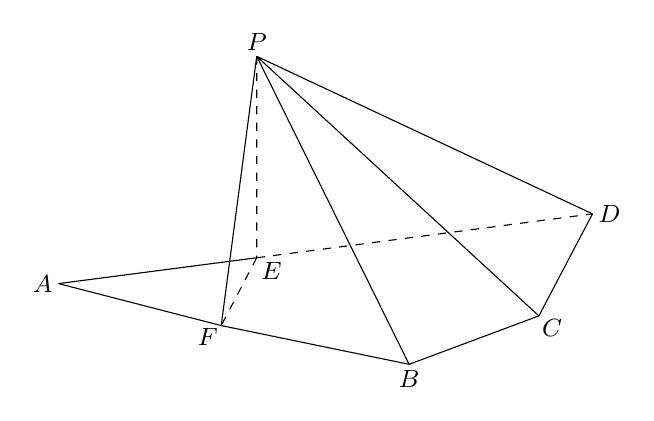
\begin{tikzpicture}[scale=0.82, font=\small]
  \coordinate (A) at (-3.07,-0.40);
  \coordinate (E) at (0,0);
  \coordinate (D) at (5.20,0.68);
  \coordinate (F) at (-0.55,-1.05);
  \coordinate (B) at (2.36,-1.65);
  \coordinate (C) at (4.37,-0.90);
  \coordinate (P) at (0,3.12);
  \draw (A) -- (E)  (A) -- (F);
  \draw (F) -- (B) -- (C) -- (D);
  \draw (P) -- (F)  (P) -- (B)  (P) -- (C)  (P) -- (D);
  \draw[dashed] (E) -- (D)  (E) -- (F)  (P) -- (E);
  \node[left, inner sep=2pt] at (A) {$A$};
  \node[below right, inner sep=1.5pt] at (E) {$E$};
  \node[right, inner sep=2pt] at (D) {$D$};
  \node[below left, inner sep=1pt] at (F) {$F$};
  \node[below, inner sep=2pt] at (B) {$B$};
  \node[below right, inner sep=1pt] at (C) {$C$};
  \node[above, inner sep=2pt] at (P) {$P$};
\end{tikzpicture}